\documentclass[12pt]{article}
\usepackage{amssymb, amsmath, amsfonts, bm, graphicx, geometry}
\usepackage{tabularx, booktabs, float, enumitem, multicol, mathtools}
\geometry{margin=1in}


\title{}
\date{}
\author{}

\begin{document}

\begin{titlepage}
    \centering
    \vspace*{1in}

    % Title of the experiment and identifying number
    {\Large\bfseries Lab 1: Verification of Ohm's Law using Resistors in Series \par}
    \vspace{1.5cm}

    % Course number
    {\large ESC 221 Basic Principles of Electrical Engineering \par}
    \vspace{2cm}

    % Author's name
    {\large \textbf{Author:} Zeshui Song \par}
    \vspace{0.5cm}

    % Names of other lab group members
    {\large \textbf{Lab Partner:}} \\
    Roy He
    \vfill

    % Date on which the lab was performed
    {\large Date Performed: February 19, 2026 \par}
    \vspace{0.8cm}

    % Name of organization sponsoring the work
    {\large Cooper Union \par}

    \vspace*{1in}
\end{titlepage}
\newpage

\section*{I. Introduction, Experimental Method and Hypotheses}
\textbf{A. Introduction}\\\\
This experiment aims to verify Ohm's Law by analyzing the relationship between voltage, current, and resistance in a series circuit.\\\\
\textbf{B. Experimental Method}\\\\
In a series circuit with two resistors (R1 and R2), a multimeter will be used to measure the voltage and current across a known resistor (R2) as the input voltage is varied. Additionally, the resistances of the resistors will be determined using the color code and verified with a multimeter to be within the manufacturer's tolerance, using the following formula for percent error:
\[\%_{Err} = \left( \frac{|Measured - Nominal|}{Nominal} \right) \times 100\%\]
\textbf{C. Hypotheses}\\\\
It is hypothesized that measured resistance values will fall within the manufacturer's stated tolerance range. For the circuit, it is expected that the current and voltage measurements will follow a linear relationship as described by Ohm's Law, $V = IR$. The predicted voltage across R2 is calculated using the voltage divider rule.
\[V_{R2} = \frac{R_2}{R_1 + R_2} \cdot V_{in}\quad[\text{V}]\]
Applying Ohm's Law, the predicted current through the resistor is:
\[I = \frac{V_{R2}}{R_2}\quad[\text{mA}]\]
\section*{II. Equipment List}
\begin{enumerate}
    \item \textbf{Digital Multimeter} \\ 
          Manufacturer: Manufacturer Name \\
          Model: Model Number
    \item \textbf{DC Power Supply} \\ 
          Manufacturer: Manufacturer Name \\
          Model: Model Number
\end{enumerate}
\section*{III. Wiring / Schematic Diagram / Procedure}
\textbf{A. Procedure}\\\\
1. Verifying Resistance
\begin{enumerate}
    \item Five resistors (1 k$\Omega$, 2.7 k$\Omega$, 3.3 k$\Omega$, 4.7 k$\Omega$, and 6.8 k$\Omega$) were selected based on their color codes, noting down their nominal resistance values and tolerance.
    \item A multimeter was set to resistance mode with an appropriate range selected to measure the resistance of each resistor (20 k$\Omega$ range). 
    \item Actual resistance values were recorded by connecting the multimeter leads across each resistor.
\end{enumerate}
2. Constructing Circuit A
\begin{enumerate}
    \item A series circuit was constructed as illustrated in Fig.~\ref{fig:Circuit_A} using a DC power supply and two $1\,\text{k}\Omega$ resistors.
    \item Resistor $R_1$ was connected between Node 1 (positive power supply terminal) and Node 2.
    \item Resistor $R_2$ was connected between Node 2 and Node 3 (ground).
\end{enumerate}
3. Constructing Circuit B
\begin{enumerate}
    \item A series circuit was constructed as illustrated in Fig.~\ref{fig:Circuit_B} using a DC power supply and a $1\,\text{k}\Omega$ resistor ($R_1$) and a $3.3\,\text{k}\Omega$ resistor ($R_2$).
    \item Resistor $R_1$ was connected between Node 1 (positive power supply terminal) and Node 2.
    \item Resistor $R_2$ was connected between Node 2 and Node 3 (ground).
\end{enumerate}
4. Measurements and Data Collection
\begin{enumerate}
    \item For each circuit, the input voltage $V_{in}$ was varied from -8 V to +8 V in increments of 2 V.
    \item For each voltage setting, the voltage across $R_2$ was measured using a multimeter connected across Node 2 and Node 3, set to voltage mode with an appropriate range (20 V range).
    \item For each voltage setting, the current through the circuit was measured by connecting the multimeter in series with the circuit at Node 2, set to current mode with an appropriate range (20 mA range).
\end{enumerate}
\newpage\noindent
\textbf{B. Schematic Diagram}
\begin{figure}[H]
    \centering
    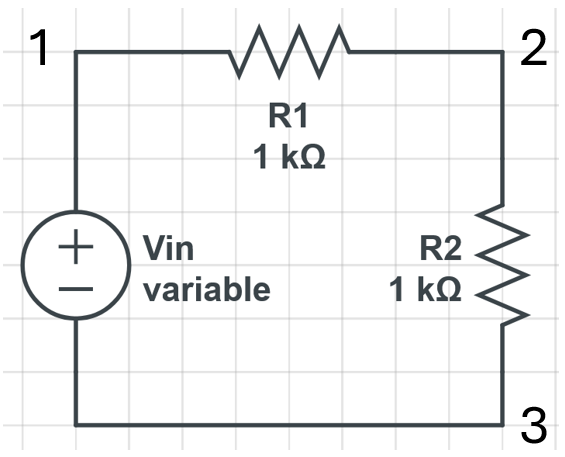
\includegraphics[width=0.4\linewidth]{Circuit A.png}
    \caption{A DC series circuit consisting of a variable voltage source $V_{in}$ and two 1\,k$\Omega$ resistors ($R_1$ and $R_2$) with labeled nodes 1, 2, and 3 for measurement points.}
    \label{fig:Circuit_A}
\end{figure}
\begin{figure}[H]
    \centering
    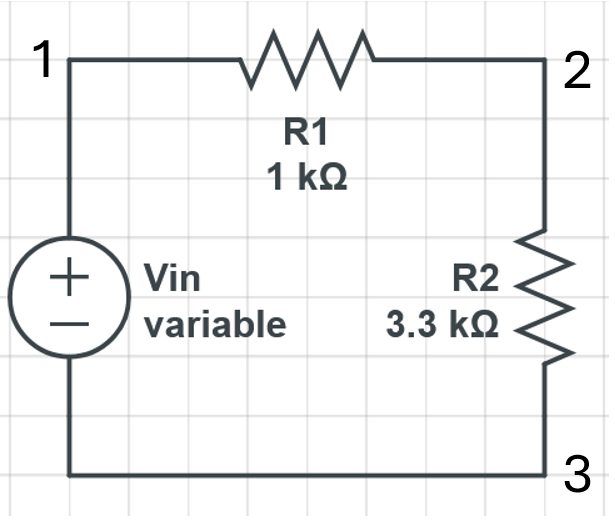
\includegraphics[width=0.4\linewidth]{Circuit B.png}
    \caption{A DC series circuit consisting of a variable voltage source $V_{in}$ and a 1\,k$\Omega$ resistor ($R_1$) and a 3.3 k$\Omega$ resistor ($R_2$) with labeled nodes 1, 2, and 3 for measurement points.}
    \label{fig:Circuit_B}
\end{figure}
\section*{IV. Results}
\begin{table}[H]
\centering
\caption{Resistor Tolerance and Measured Values}
\begin{tabularx}{\linewidth}{*{6}{>{\centering\arraybackslash}X}}
\toprule
\textbf{Resistor (k$\Omega$)} & \textbf{Nominal Value (k$\Omega$)} & \textbf{Tolerance (\%)} & \textbf{Measured Value (k$\Omega$)} & \textbf{In Spec?} & \textbf{\% Error} \\
\midrule
1   & 1   & 1  & 0.99 & Yes & 1.00 \\
2.2 & 2.2 & 1  & 2.18 & Yes & 0.91 \\
3.3 & 3.3 & 5  & 3.25 & Yes & 1.52 \\
4.7 & 4.7 & 5  & 4.65 & Yes & 1.06 \\
6.8 & 6.8 & 5  & 6.72 & Yes & 1.18 \\
\bottomrule
\end{tabularx}
\end{table}
\begin{table}[H]
\centering
\caption{Circuit A (R$_2$ = 1 k$\Omega$) Experimental Data}
\begin{tabularx}{\linewidth}{*{5}{>{\centering\arraybackslash}X}}
\toprule
\textbf{V$_{in}$ (V)} & \textbf{Predicted Current (mA)} & \textbf{Predicted Voltage (V)} & \textbf{Measured Current (mA)} & \textbf{Measured Voltage (V)} \\
\midrule
 2  &  1.00 &  1.00 &  1.00 &  1.00 \\
 4  &  2.00 &  2.00 &  1.96 &  1.96 \\
 6  &  3.00 &  3.00 &  2.94 &  2.96 \\
 8  &  4.00 &  4.00 &  3.98 &  4.00 \\
-2  & -1.00 & -1.00 & -1.00 & -1.00 \\
-4  & -2.00 & -2.00 & -2.03 & -1.97 \\
-6  & -3.00 & -3.00 & -2.80 & -2.74 \\
-8  & -4.00 & -4.00 & -4.09 & -4.00 \\
\bottomrule
\end{tabularx}
\end{table}
\begin{table}[H]
\centering
\caption{Circuit B (R$_2$ = 3.3 k$\Omega$) Experimental Data}
\begin{tabularx}{\linewidth}{*{5}{>{\centering\arraybackslash}X}}
\toprule
\textbf{V$_{in}$ (V)} & \textbf{Predicted Current (mA)} & \textbf{Predicted Voltage (V)} & \textbf{Measured Current (mA)} & \textbf{Measured Voltage (V)} \\
\midrule
 2  &  0.4651 &  1.5349 &  0.46 &  1.53 \\
 4  &  0.9302 &  3.0698 &  0.97 &  3.11 \\
 6  &  1.3953 &  4.6047 &  1.42 &  4.59 \\
 8  &  1.8605 &  6.1395 &  1.90 &  5.92 \\
-2  & -0.4651 & -1.5349 & -0.47 & -1.52 \\
-4  & -0.9302 & -3.0698 & -0.95 & -3.05 \\
-6  & -1.3953 & -4.6047 & -1.44 & -4.62 \\
-8  & -1.8605 & -6.1395 & -1.92 & -6.17 \\
\bottomrule
\end{tabularx}
\end{table}
\begin{figure}[H]
    \centering
    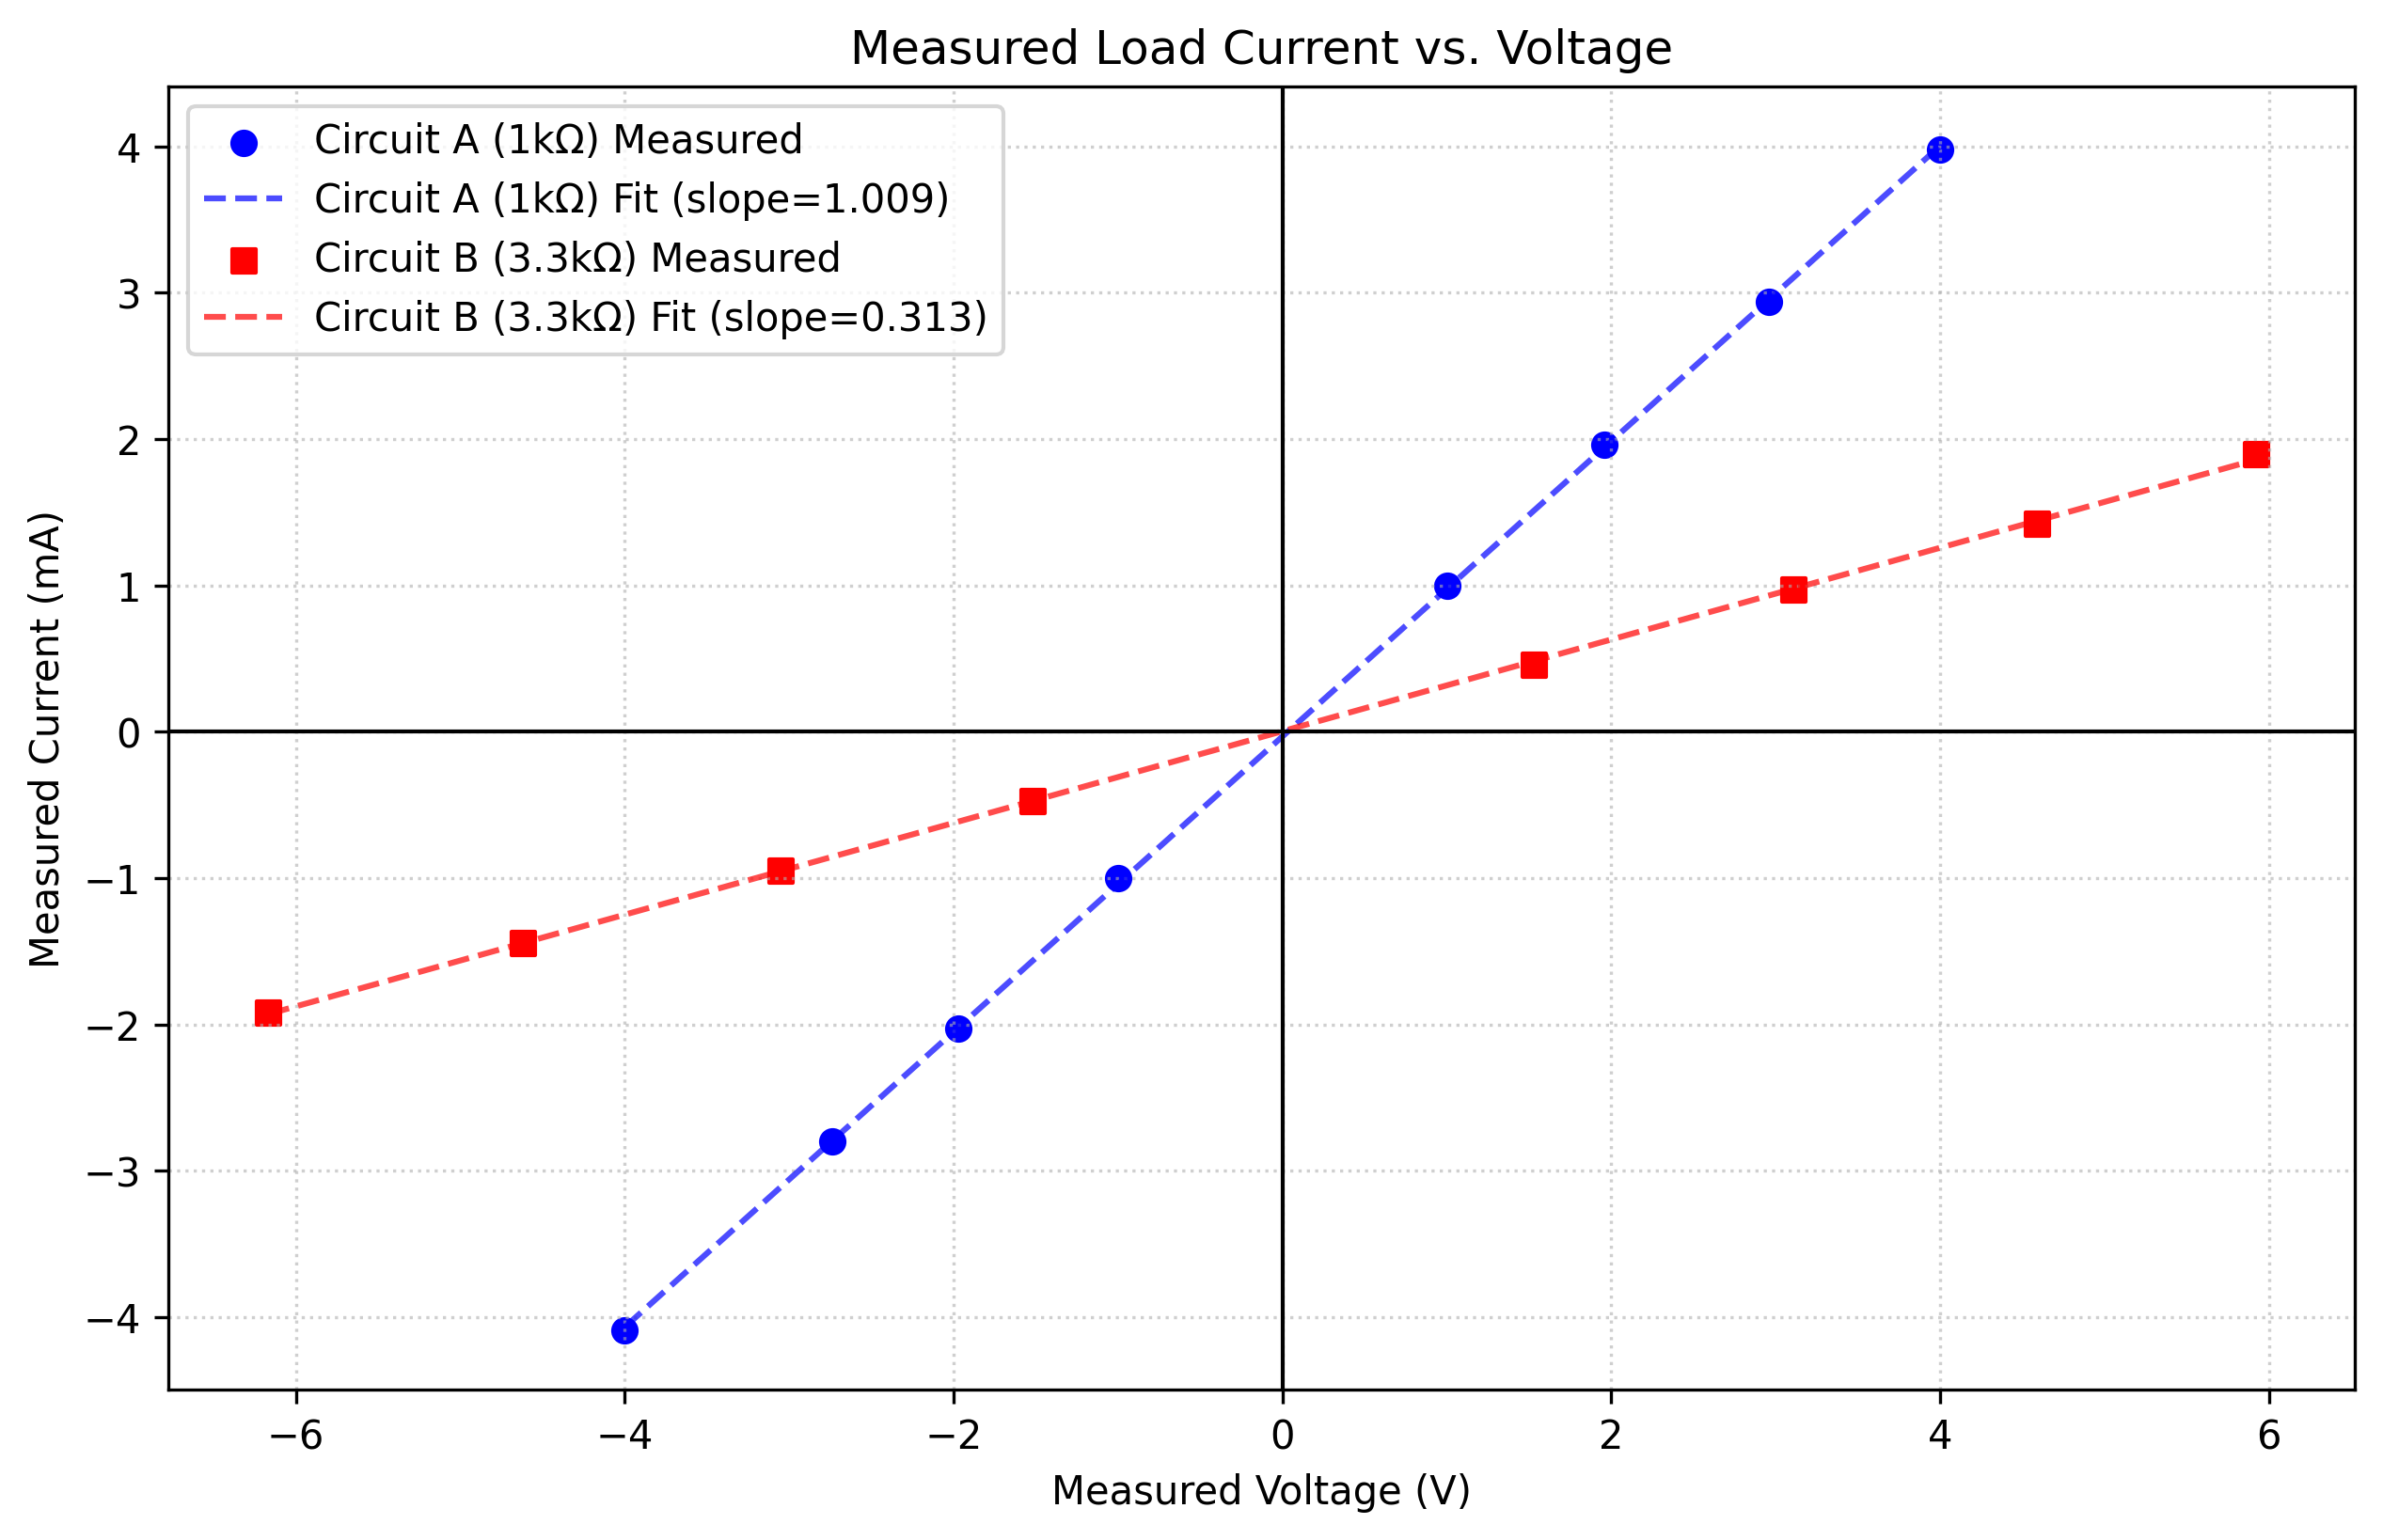
\includegraphics[width=1\linewidth]{Plot.png}
    \caption{Comparison of measured current (mA) vs. voltage (V) for Circuit A ($R_2$ = 1 k$\Omega$) and Circuit B ($R_2$ = 3.3 k$\Omega$), showing linear Ohm’s Law behavior and calculated best-fit lines.}
    \label{fig:Plot}
\end{figure}
\section*{V. Discussion, Analysis and Concluding Statements}
\textbf{A. Resistor Tolerances}\\\\
All selected resistors (1 k$\Omega$, 2.2 k$\Omega$, 3.3 k$\Omega$, 4.7 k$\Omega$, and 6.8 k$\Omega$) were found to be within their manufacturer stated tolerance ranges as seen in Table~1. The calculated percent error for all components remained low, with the highest error being 1.52\% for the 3.3 k$\Omega$ resistor. This indicates that the resistors used in the experiment were of good quality and suitable for verifying Ohm's Law.\\\\
\textbf{B. Verification of Ohm's Law}\\\\
The relationship between current and voltage for both Circuit A and Circuit B was found to be linear, as shown in Figure~\ref{fig:Plot}.
\begin{itemize}
    \item \textbf{Circuit A Analysis:} For $R_2 = 1\,\text{k}\Omega$ in Table 2, the measured current and voltage closely matched the predicted values. For example, at $V_{in} = 8\,\text{V}$, the measured voltage across $R_2$ was 4.00~V, and the measured current was 3.98~mA, aligning with the predicted values.
    
    \item \textbf{Circuit B Analysis:} For $R_2 = 3.3\,\text{k}\Omega$ in Table 3, the measured values followed the voltage divider and Ohm's Law predictions with similar consistency. At $V_{in} = 4\,\text{V}$, the measured voltage was 3.11~V compared to the predicted 3.0698~V.
\end{itemize}
\textbf{B. Slope and Significance}\\\\
The slope of the current versus voltage plot in Figure~\ref{fig:Plot} represents the conductance ($G$) of the load resistor, which is the reciprocal of the resistance ($G = 1/R$).

\begin{itemize}
    \item In \textbf{Circuit A}, the best-fit slope was 1.009, which corresponds to a resistance of approximately 
    $1/1.009 \approx 0.991\,\text{k}\Omega$.
    
    \item In \textbf{Circuit B}, the best-fit slope was 0.313, corresponding to a resistance of approximately 
    $1/0.313 \approx 3.195\,\text{k}\Omega$.
\end{itemize}
These experimental slopes closely align with the measured resistance values recorded in Table~1, confirming the Ohm's Law relationship $I = V/R$.\\\\
\textbf{C. Conclusion}\\\\
This experiment demonstrated that the current through a resistor is directly proportional to the voltage across it. Small discrepancies between predicted and measured values can be attributed to the tolerances of the resistors and minor fluctuations in $V_{in}$ from the DC power supply. Overall, the hypotheses were supported, and the validity of Ohm’s Law was confirmed through the experimental data collected in both circuits.

\end{document}